\documentclass[11pt]{article}
\usepackage{amsmath, amssymb, amsthm}
\usepackage[retainorgcmds]{IEEEtrantools}

\usepackage[pdftex]{graphicx}
\usepackage{tikz}
\usepackage{circuitikz}
\usetikzlibrary{intersections}

\usepackage{fancyhdr}

%Format stuff
\pagestyle{fancy}
\headheight 35pt

%Header info
\chead{\Large \textbf{EM Waves}}
\lhead{}
\rhead{}

\begin{document}
\section{Maxwell's Equations in Integral Form}
	\subparagraph{Gauss's Law} Gauss's law of electricity relates electric flux through a surface to the charge enclosed within the surface. Gauss's law of magnetism states that the magnetic flux through any closed surface must be 0 (i.e. no magnetic monopoles exist).
	\begin{equation}
		\int_S \vec{E} \cdot \hat{n} dA = \frac{Q_{enclosed}}{\varepsilon_0}
	\end{equation}
	\begin{equation}
		\int_S \vec{B} \cdot \hat{n} dA = 0
	\end{equation}
	
	\subparagraph{Faraday's Law} Changing magnetic flux induces an electric field.
	\begin{equation}
		\oint \vec{E} \cdot d\vec{l} = \frac{-d\Phi_B}{dt}
	\end{equation}
	
	\subparagraph{Ampere's Law} Current in a wire induces a magnetic field. Note the extra \textbf{displacement current} term to account for the possibility of a discontinuity in the path (e.g. a capacitor).
	\begin{equation}
		\oint \vec{B} \cdot d\vec{l} = \mu_0 \left( I + \varepsilon_0 \frac{d\Phi_E}{dt} \right)
	\end{equation}
	
	\subsection{Wave Equation}
		To derive the wave equation for EM waves from the integral forms of Maxwell's equations, first imagine a vertical electric field in the x-y plane that induces a magnetic current in the z-direction:
		\begin{center}
		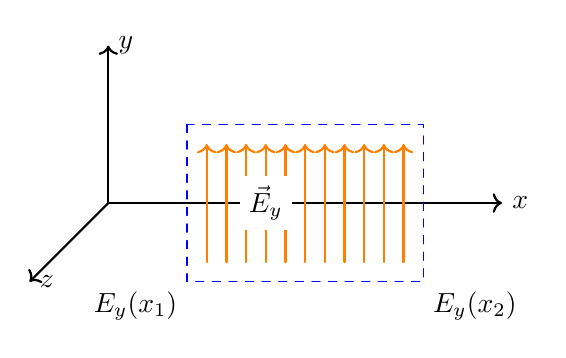
\begin{tikzpicture}
			[scale=1,line cap=round,
			%Styles
			axes/.style=,
			important line/.style={very thick},
			information text/.style={rounded corners,fill=red!10,inner sep=1ex},
			dot/.style={circle,inner sep=1pt,fill,label={#1},name=#1}			
			]
			
			%Colors
			\colorlet{anglecolor}{green!50!black}	%angle arcs/lines
			
			%The graphic
			\draw[->,thick] (0, 0) -- (0, 2) node[right] {$y$};
			\draw[->,thick] (0, 0) -- (5, 0) node[right] {$x$};
			\draw[->,thick] (0, 0) -- (-1, -1) node[right] {$z$};
			
			\draw[blue,dashed] (1, 1) rectangle (4, -1);
			\draw[orange,->,thick] (1.25, -.75) -- (1.25, .75);
			\draw[orange,->,thick] (1.5, -.75) -- (1.5, .75);
			\draw[orange,->,thick] (1.75, -.75) -- (1.75, .75);
			\draw[orange,->,thick] (2, -.75) -- (2, .75);
			\draw[orange,->,thick] (2.25, -.75) -- (2.25, .75);
			\draw[orange,->,thick] (2.5, -.75) -- (2.5, .75);
			\draw[orange,->,thick] (2.75, -.75) -- (2.75, .75);
			\draw[orange,->,thick] (3, -.75) -- (3, .75);
			\draw[orange,->,thick] (3.25, -.75) -- (3.25, .75);
			\draw[orange,->,thick] (3.5, -.75) -- (3.5, .75);
			\draw[orange,->,thick] (3.75, -.75) -- (3.75, .75);
			
			\node[fill=white] at (2, 0) {$\vec{E}_y$};
			\node[below right] at (4, -1) {$E_y(x_2)$};
			\node[below left] at (1, -1) {$E_y(x_1)$};
		\end{tikzpicture}
		\end{center}
		
		Use Faraday's Law on the enclosing rectangle counterclockwise:
		\begin{IEEEeqnarray}{rCl}
			\oint \vec{E} \cdot d\vec{l} & = & (E_y(x_2) - E_y(x_1)) \Delta y\\
			\oint \vec{E} \cdot d\vec{l} & \approx & \frac{\partial E_y}{\partial x}\Delta x \Delta y
		\end{IEEEeqnarray}
		Substitute into Faraday's Law and transform the RHS:
		\begin{IEEEeqnarray}{rCl}
			\frac{\partial E_y}{\partial x}\Delta x \Delta y & = & -\frac{d\Phi_B}{dt}\\
			\frac{\partial E_y}{\partial x}\Delta x \Delta y & = & -\frac{d}{dt}\oint \vec{B} \cdot \hat{n} dA\\
			\frac{\partial E_y}{\partial x}\Delta x \Delta y & \approx & -\frac{d}{dt} (B_z \Delta x \Delta y)\\
			\frac{\partial E_y}{\partial x} & = & -\frac{\partial B_z}{\partial t}
		\end{IEEEeqnarray}
		
		Now imagine a magnetic field in the x-z plane, inducing an electric field in the y-direction:

		\begin{center}
		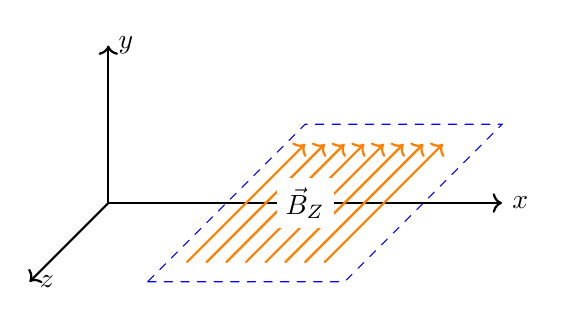
\begin{tikzpicture}
			[scale=1,line cap=round,
			%Styles
			axes/.style=,
			important line/.style={very thick},
			information text/.style={rounded corners,fill=red!10,inner sep=1ex},
			dot/.style={circle,inner sep=1pt,fill,label={#1},name=#1}			
			]
			
			%Colors
			\colorlet{anglecolor}{green!50!black}	%angle arcs/lines
			
			%The graphic
			\draw[->,thick] (0, 0) -- (0, 2) node[right] {$y$};
			\draw[->,thick] (0, 0) -- (5, 0) node[right] {$x$};
			\draw[->,thick] (0, 0) -- (-1, -1) node[right] {$z$};
			
			\draw[dashed,blue,->] (.5, -1) -- (3, -1) -- (5, 1) -- (2.5, 1) -- cycle;
			\draw[orange,->,thick] (1, -.75) -- (2.5, .75);
			\draw[orange,->,thick] (1.25, -.75) -- (2.75, .75);
			\draw[orange,->,thick] (1.5, -.75) -- (3, .75);
			\draw[orange,->,thick] (1.75, -.75) -- (3.25, .75);
			\draw[orange,->,thick] (2, -.75) -- (3.5, .75);
			\draw[orange,->,thick] (2.25, -.75) -- (3.75, .75);
			\draw[orange,->,thick] (2.5, -.75) -- (4, .75);
			\draw[orange,->,thick] (2.75, -.75) -- (4.25, .75);
			
			\node[fill=white] at (2.5, 0) {$\vec{B}_Z$};
		\end{tikzpicture}
		\end{center}
		
		By the same process as above except with Ampere's Law in a vacuum,
		\begin{equation}
			\frac{\partial B_z}{\partial x} = -\mu_0 \varepsilon_0 \frac{\partial E_y}{\partial t}
		\end{equation}
		
		Taking a further partial with respect to $x$ of the equation derived from applying Faraday's Law gives the wave equation for EM waves:
		\begin{equation}
			\frac{\partial^2 E_y}{\partial x^2} = \mu_0 \varepsilon_0 \frac{\partial^2 E_y}{\partial t^2}
		\end{equation}
		The EM field allows propagation of waves at the speed of light, as
		\begin{equation}
			v_p = \frac{1}{\sqrt{\mu_0 \varepsilon_0}} = c
		\end{equation}
		
\section{Maxwell's Equations in Differential Form}
	\subparagraph{Gauss's Law} Apply Gauss's Theorem to the integral form of Gauss's Law to get
	\begin{equation}
		\nabla \cdot \vec{E} = \frac{\rho}{\varepsilon_0}
	\end{equation}
	\begin{equation}
		\nabla \cdot \vec{B} = 0
	\end{equation}
	where $\rho$ is the charge density, $Q = \int \rho dV$. Note that in a vacuum,
	\begin{equation}
		\nabla \cdot \vec{E} = 0
	\end{equation}
	
	\subparagraph{Faraday's Law} Apply Stoke's Theorem to the integral form.
	\begin{equation}
		\nabla \times \vec{E} = -\frac{\partial \vec{B}}{\partial t}
	\end{equation}
	
	\subparagraph{Ampere's Law} Apply Stoke's Theorem on the integra form.
	\begin{equation}
		\nabla \times \vec{B} = \mu_0 \vec{J} + \mu_0 \varepsilon_0 \frac{\partial \vec{E}}{\partial t}
	\end{equation}
	where $\vec{J}$ is the current density, or the current per unit area perpendicular to the surface. Note that in a vacuum,
	\begin{equation}
		\nabla \times \vec{B} = \mu_0 \varepsilon_0 \frac{\partial \vec{E}}{\partial t}
	\end{equation}
	
	The forms of Maxwell's equations in a vacuum show that the only thing that can create a magnetic/electric field is change in the other. The resulting field circulates due to the curl.
	
	\subsection{Wave Equation}
		Start with Faraday's Law and take a second curl:
		\begin{IEEEeqnarray}{rCl}
			\nabla \times \vec{E} & = & -\frac{\partial \vec{B}}{\partial t}\\
			\nabla \times (\nabla \times \vec{E}) & = & \nabla \times \left( -\frac{\partial \vec{B}}{\partial t} \right)\\
			\nabla(\nabla \cdot \vec{E}) - \nabla^2 \vec{E} & = & -\frac{\partial}{\partial t} (\nabla \times \vec{B})
		\end{IEEEeqnarray}
		Remember that in a vacuum, $\nabla \cdot \vec{E} = 0$, and apply Ampere's Law in a vacuum on the RHS of the equation to get the wave equation for EM waves,
		\begin{equation}
			\nabla^2\vec{E} = \mu_0 \varepsilon_0 \frac{\partial^2 \vec{E}}{\partial t^2}
		\end{equation}
		Similarly for the magnetic field,
		\begin{equation}
			\nabla^2\vec{B} = \mu_0 \varepsilon_0 \frac{\partial^2 \vec{B}}{\partial t^2}
		\end{equation}
		
\section{Plane Wave Solution}
	A plane wave solution to the wave equation for EM waves can be written as
	\begin{equation}
		\vec{E}(z, t) = \vec{E}_0 e^{i(kz-\omega t)}
	\end{equation}
	\begin{equation}
		\vec{B}(z, t) = \vec{B}_0 e^{i(kz-\omega t)}
	\end{equation}
	
	Maxwell's equations specify some other constraints for the plane wave. Specifically, that $\vec{E}$ and $\vec{B}$ are orthogonal to both each other and the direction of travel and are in phase. Specifically, if $\hat{z}$ is the direction of travel, then
	\begin{equation}
		\vec{B}_0 = \frac{k}{\omega}(\hat{z} \times \vec{E}_0)
	\end{equation}
	or
	\begin{equation}
		\hat{z} \times \vec{E}_0 = c\vec{B}_0
	\end{equation}
	
	For a more general plane wave solution, define $\vec{k}$ as the direction of travel, $\hat{n}$ as some unit vector perpendicular to $\vec{k}$, and $\vec{r}$ as an arbitrary position vector. Then the plane wave solution can be written as
	\begin{equation}
		\vec{E}(\vec{r}, t) = |\vec{E}_0| \hat{n} e^{i(\vec{k} \cdot \vec{r} - \omega t)}
	\end{equation}
	\begin{equation}
		\vec{B}(\vec{r}, t) = \frac{1}{c}|\vec{E}_0|(\hat{k} \times \hat{n})e^{i(\vec{k} \cdot \vec{r} - \omega t)}
	\end{equation}
	
	\subsection{Poynting Vector}
		Remember the energy densities of electric and magnetic fields:
		\begin{IEEEeqnarray}{rCl}
			u_E & = & \frac{1}{2} \varepsilon_0 |\vec{E}|^2\\
			u_B & = & \frac{1}{2} \mu_0 |\vec{B}|^2
		\end{IEEEeqnarray}
		
		Substituting the plane wave solutions gives symmetrical energy densities, so the total energy density of the system is
		\begin{equation}
			u = \varepsilon_0 |\vec{E}|^2
		\end{equation}
		
		Define the Poynting vector as
		\begin{equation}
			\vec{S} = \frac{1}{\mu_0} \vec{E} \times \vec{B}
		\end{equation}
		pointing in the direction of travel, which after substitution gives
		\begin{equation}
			\vec{S} = cu \ \hat{z}
		\end{equation}
		The Poynting vector has units of velocity by energy density pointing in the direction of travel and represents the amount of energy transmitted by the EM waves through a plane.
		
		Note the time average of $\vec{S}$ is
		\begin{equation}
			<\vec{S}> = I = \frac{1}{2}c\varepsilon_0 |\vec{E}_0|^2
		\end{equation}
		
\section{Dielectrics}
	Maxwell's equations remain the same in a dielectric medium except $\mu_0$ and $\varepsilon_0$ are replaced by $\mu$ and $\varepsilon$ specific to the medium. Define the \textbf{index of refraction} as
	\begin{equation}
		n = \frac{c}{v_p} = \sqrt{\frac{\varepsilon \mu}{\varepsilon_0 \mu_0}}
	\end{equation}
	In most simple dielectrics, $\mu \approx \mu_0$, so $n > 1$.
	
	If an incident EM wave traveling through one dielectric medium meets the boundary to another dielectric medium, it will be partially reflected and transmitted through. The amplitudes of the reflected and transmitted waves can be described by
	\begin{equation}
		E_{0R} = \frac{\mu_2 v_2 - \mu_1 v_1}{\mu_2 v_2 + \mu_1 v_1} E_{0I}
	\end{equation}
	\begin{equation}
		E_{0T} = \frac{2}{\mu_2 v_2 + \mu_1 v_1} E_{0I}
	\end{equation}
	
	Now define the impedance for EM waves as
	\begin{equation}
		Z = \mu v = \sqrt{\frac{\mu}{\varepsilon}}
	\end{equation}
	Note that the impedance of free space is 376.7$\Omega$. This yields the familiar expressions
	\begin{equation}
		E_{0R} = \frac{Z_2 - Z_1}{Z_1 + Z_2} E_{0I}
	\end{equation}
	\begin{equation}
		E_{0T} = \frac{2}{Z_1 + Z_2} E_{0I}
	\end{equation}
	Because $\mu \approx \mu_0$ in most dielectrics, we can express the intensity of the reflected wave in terms of the intensity of the incident wave:
	\begin{equation}
		I_{reflected} = \left( \frac{n_1 - n_2}{n_1 + n_2} \right)^2 I_{incident}
	\end{equation}
%	\begin{center}
%	\begin{tikzpicture}
%		[scale=3,line cap=round,
%		%Styles
%		axes/.style=,
%		important line/.style={very thick},
%		information text/.style={rounded corners,fill=red!10,inner sep=1ex},
%		dot/.style={circle,inner sep=1pt,fill,label={#1},name=#1}			
%		]
%		
%		%Colors
%		\colorlet{anglecolor}{green!50!black}	%angle arcs/lines
%		
%		%The graphic
%	\end{tikzpicture}
%	\end{center}

%	\begin{figure}[htb]
%		\centering
%		\includegraphics[width=0.8\textwidth]{filename.eps}
%		\caption{Caption.}
%		\label{fig:figure}
%	\end{figure}

%		\def\enotesize{\normalsize}
%		\theendnotes
\end{document}